\versoimage
\chapter{TLS Identification In \lin{3D}}\label{ch:threedee}
\loftchap{TLS Identification In \lin{3D}}
\chapterprecis{That's some fancy lookin' graphs you got there.}

\thought{Memory limitations were the greatest} concern with the implementation of the direct diagonalisation approach discussed in the previous chapter.
The \lin{2+1D} framework may capture all relevant physics and therefore the need to extend the system to a complete \lin{3D} may be moot.
However, the only way to verify this statement is to compare a \lin{3D} representation of the TLS model with its \lin{2+1D} counterpart.

In this chapter we focus on a delocalised oxygen TLS model in three spatial dimensions.
\Cref{sec:ddiagthree} discusses the pitfalls and concerns of extending the current \lin{2+1D} to \lin{3D} at low resolution such that the solution fits into memory.
As this method can not be trusted to yield accurate results, we introduce an alternative method in \cref{sec:meth3d} which can be executed on highly distributed clusters over many CPU cores.

\Crefrange{sec:aloal3d}{sec:jjtls} discuss the capabilities and results that can be obtained with this method.
Starting in \cref{sec:aloal3d} a comparison of the Al--O--Al chain discussed in \cref{sec:bonds} is examined, followed by descriptions of the wavefunctions exhibited by various atomic configurations, some of which can be identified as A and B type defects in \cref{sec:orbitals,sec:atype3d}.
\Cref{sec:corundum} generates clusters of atoms surrounding an oxygen vacancy defect in \ce{Al_2O_3}, then using the same method \cref{sec:jjtls} calculates TLS properties in junction models constructed in \cref{ch:junctions}.
Finally, a small summary of the alternate method is given in \cref{sec:summary3d}.

\section[Extending Direct Diagonalisation To \lin{3D}]{Extending Direct Diagonalisation To 3D}\label{sec:ddiagthree}

Constructing the Hamiltonian $H$ \cref{eq:OHam} in three dimensions is a quick extension to the two dimension block matrix solution \cref{eq:h2d}
\begin{equation}
H = \left[H_x \otimes (\mathbb{I}_y \otimes \mathbb{I}_z)\right] + \left[(\mathbb{I}_x \otimes H_y) \otimes \mathbb{I}_z\right] + \left[(\mathbb{I}_x \otimes \mathbb{I}_y) \otimes H_z\right].
\label{eq:h3d}
\end{equation}

The triviality of this extension stops there though.
As shown in \cref{sec:hmax}, the maximum acceptable step size one can apply to the model is $h_{max} = 2^{-3} \simeq 0.125$ Å.
Larger step values will introduce invalid truncation error into the solution and cannot be treated as valid solutions.
The same machine used to calculate the values required for \cref{fig:econv} and the associated discussion is not capable of fitting a \lin{3D} calculation into its memory and swap space with a step size any smaller than $h \approx 0.7$ Å.

Additionally, many excited state wavefunctions exhibit sign changes on scales much less than $0.7$ Å, provoking another systemic error: the selection of an incorrect excited state value which does not have such a rapid sign change in the region.

\section{An Alternative Method}\label{sec:meth3d}

\citeauthor{Strickland2010} put forward a method which exploits a Wick-rotated time-dependent Schr\"{o}dinger equation to solve for time-independent solutions in three dimensions~\cite{Strickland2010}.

\Cref{eq:tisemat} ignores any time evolution of our TLS model, although the general case \cref{eq:tdse} includes this description.
Wick rotations~\cite{Wick1954} are primarily used to find solutions to Minkowski space problems by an Euclidean space mapping.
Here we can use the same method to transfer our Schr\"{o}dinger equation to an imaginary time basis $t=i\tau$ \cref{eq:tdseit}
\begin{align}
i \hbar \frac{\partial}{\partial t}\Psi(\mathbf{r},t) &= H\Psi(\mathbf{r},t)\label{eq:tdse}\\
\Rightarrow - \hbar \frac{\partial}{\partial \tau}\Psi(\mathbf{r},\tau) &= H\Psi(\mathbf{r},\tau),\label{eq:tdseit}
\end{align}

which yields a general solution to the wavefunctions
\begin{equation}
\Psi(\mathbf{r},\tau) = \sum_{n=0}^\infty a_n\psi_n(\mathbf{r})e^{-E_n \tau}.\label{eq:psitau}
\end{equation}

Here, ${a_n}$ are coefficients based on initial conditions of the system where $n=0$ indicates the ground state, $n=1$ the first excited state \etc\ and $E_n$ is the corresponding eigenenergy.
As $E_0 < E_1 < E_2 < \ldots$, evolving \cref{eq:psitau} to large imaginary time will provide a good approximation to the ground state influenced by the time-independent potential $V(\mathbf{r})$.

This solution is obtained by numerically approximating the spatial derivatives with finite differences.
For both stability and precision, we descritise the space using the $7$-point central difference method discussed comprehensively in \cref{ch:tls}.

\subsection{Gram-Schmidt Procedure}\label{sec:gsp}

One important property of a hermitian operator (in our case $H$), is orthogonality. That is: a system's eigenfunctions belong to distinct eigenvalues which are orthogonal.
The proof of this theorem neglects degenerate states, although it can be shown that any linear combination of eigenfunctions which share the same eigenvalue are indeed eigenfunctions of the system.

Using the Gram-Schmidt orthogonalisation procedure \cite{Gram1883, Schmidt1907}, orthogonal eigenfunctions within a degenerate subspace can be constructed; \textit{chosen} to be orthogonal to the system's basis.

Consider a non-orthonormal basis of vectors $\ket{a_1}, \ket{a_1}, \ldots \ket{a_n}$.
A new, orthonormal basis for these vectors can by found be first normalising the initial vector
\begin{equation}
\ket{a^\prime_1} = \frac{\ket{a_1}}{\norm{a_1}},
\end{equation}

then finding the projection of the second vector along the first and subtracting it.
This vector is orthogonal to $\ket{a^\prime_1}$ and normalising it obtains
\begin{equation}
\ket{a^\prime_2} = \frac{\ket{a_2}-\ket{a^\prime_1}\bket{a^\prime_1}{a_2}}{\norm[\big]{\ket{a_2}-\ket{a^\prime_1}\bket{a^\prime_1}{a_2}}}.
\end{equation}

Similarly, the third vector requires the same treatment, although projections along both $\ket{a^\prime_1}$ and $\ket{a^\prime_2}$ are needed
\begin{equation}
\ket{a^\prime_3} = \frac{\ket{a_3}-\ket{a^\prime_1}\bket{a^\prime_1}{a_3}-\ket{a^\prime_2}\bket{a^\prime_2}{a_3}}{\norm[\big]{\ket{a_3}-\ket{a^\prime_1}\bket{a^\prime_1}{a_3}-\ket{a^\prime_2}\bket{a^\prime_2}{a_3}}}.\label{eq:gs3ex}
\end{equation}

This process is repeated until the orthonormal vector $\ket{a^\prime_n}$ is calculated.

Applying this procedure to our particular case, consider a converged, orthonormal ground state $\ket{\psi_0}$ and an initial, non-orthonormal guess for the first excited state $\ket{\psi^\prime_1}$.
Subtracting the projection of the excited state along the ground state from the initial guess yields a vector orthogonal to the ground state
\begin{equation}
\lvert\widetilde{\psi}^\prime_1\rangle = \ket{\psi^\prime_1}-\ket{\psi_0}\bket{\psi_0}{\psi^\prime_1}.
\end{equation}
This resultant vector can then be normalised and evolved through the same process as the ground state (\ie the evolution of \labelcref{eq:psitau} to large imaginary times) until convergence is achieved.
Similarly, the second excited state requires the same treatment, although projections along both $\ket{\psi_0}$ and $\ket{\psi_1}$ are needed.

\subsection{Implementation}

Further theoretical discussion and a link to a rudimentary code base which implements the method can be found in \onlinecite{Strickland2010}.
This software discretises over a 3-point central difference solution and does not iteratively solve higher order excited state wavefunctions, just merely approximates the first excited state.

The results obtained within this chapter were calculated using a highly modified fork of the original software specifically designed for this thesis.
An active repository of this code can be found via \onlinecite{DuBois2015c} and may be packaged for general release in the future.

\section[Perturbed Lattice Representation in \lin{3D}]{Perturbed Lattice Representation in 3D}\label{sec:aloal3d}

With this new approach, we have the capability to investigate oxygen delocalisation in \lin{3D}, using realistic atomic positions within an amorphous layer of $\ce{AlO_x}$.
However this generates an extensive state space, and whilst a highly distributed computing cluster can be invoked to share the load, phase maps similar to those in \cref{ch:lowdims} are still impractical with the added time burden required for accurate calculations ($\sim 200$ hours for 6 states in one spatial configuration).

Hence we start this investigation using a simple three atom system comprising of an oxygen atom and a confining aluminium pair $\abs{X}$, representing a perturbed crystalline system as \cref{sec:bonds} did with the direct diagonalisation approach.
An eigenspectrum is generated by increasing or decreasing the pair separation distance from the corrundum lattice distance $1.85$ \AA\ using the ground and five lowest excited energy levels of this system, depicted in \cref{fig:spect3d} (for comparison with the \lin{2D} model, see \cref{fig:spectrum}).

\begin{figure}[htp]
  \resizebox{0.9\textwidth}{!}{\includestandalone{figures/spect3d}}
  \caption[Eigenspectrum]{\label{fig:spect3d}Eigenspectrum of a three atom system Al--O--Al, over a varying distance separation. Each excited state has been normalised with the ground state, which shows a clear $E_{01}$ degeneracy at large separation distance---indicative of a B type defect. An intermediate region exists as the separation distance decreases, which is approximately centered about the optimal Al--O bond distance of corundum ($1.85$ \AA). At small separation distances, the eigenspectrum is distributed over comparatively small energy levels, but is not degenerate (see \cref{fig:lift}).}
\end{figure}

In this figure an (an)harmonic division about $\abs{X} \sim 1.85$ \AA\ separates two regions with dissimilar properties.
In the region where $\abs{X} > 1.95$ \AA, a degenerate $E_{01}$ is observed and as the separation distance has increased, can be identified as a possible B type defect (see \cref{fig:sio2}).
The second region ($\abs{X} < 1.55$ \AA) has a tightly bound eigenspectrum compared to the rest of the map although this yields no degeneracy.

In three dimensions, the potential minima manifests as a sphere around the location of an atom. As a consequence the three atom Al--O--Al chain produces a unique, rotationally symmetric ground state which is reminiscent of an oxygen interstitial defect in crystalline germanium~\cite{Artacho1995} and depicted in \cref{fig:liftab}
Comparatively, this region in the \lin{2D} case indicated the presence of an A type defect, as the \lin{2D} potential minima ring would be projected onto a plane, collapsing a degree of freedom.

Two other observations concerning the \lin{2D} to \lin{3D} transition is the dramatically reduced total energy values as wavefunctions are no longer artificially confined, and the higher excited states in the B type region now exhibit a quad degeneracy rather than two split doubly degenerate pairs---again because the states are not artificially confined in the extra dimension.

\begin{figure}[htp]
  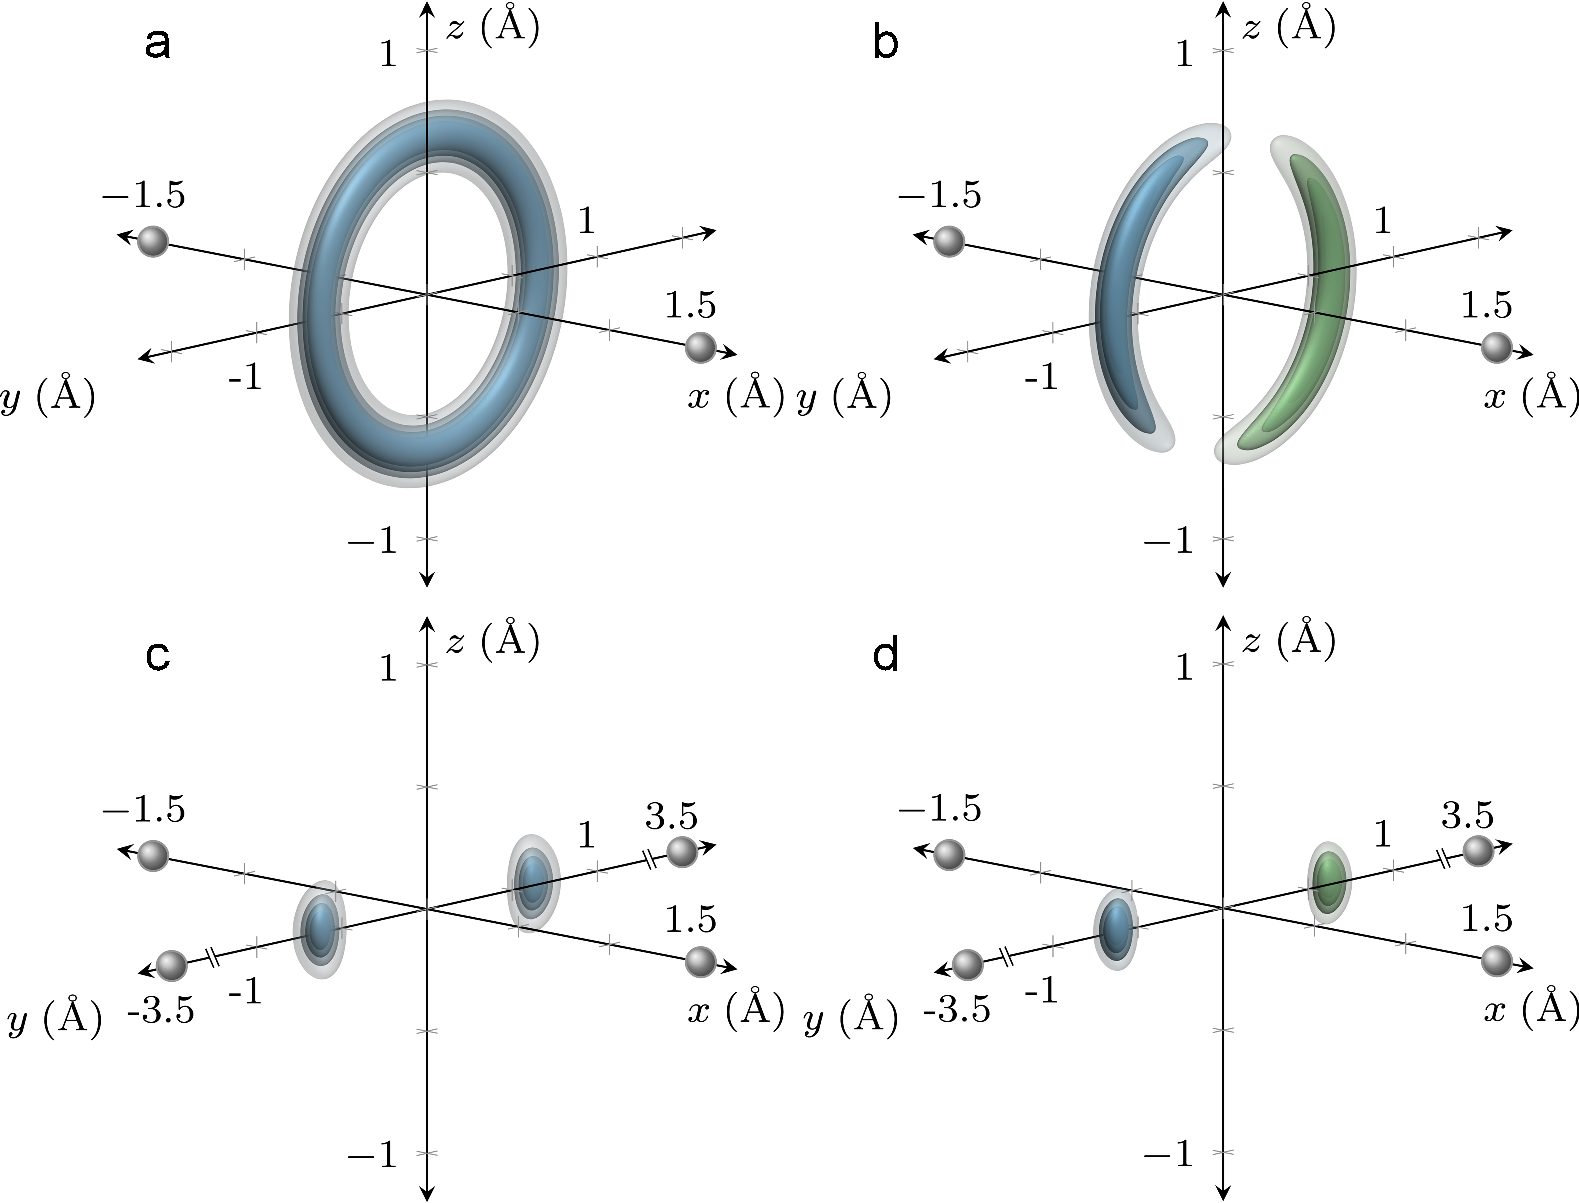
\includegraphics[width=\textwidth]{figures/lift}
  \caption[ground]{\label{fig:lift}\label[figureab]{fig:liftab}\label[figurecd]{fig:liftcd}Ground (left) and first excited (right) state wavefunctions of an Al--O--Al chain with $\abs{X} = 1.5$ \AA (aluminium atoms are depicted as \resizebox{0.5em}{!}{\includegraphics{figures/aluminium}}). Top axes show a unique ground state, the $E_{12}$ pair is degenerate in this case. Two more aluminium atoms are introduced at $\abs{Y} = 3.5$ \AA\ on the bottom axes, which causes degeneracy in the $E_{01}$ pair.}
\end{figure}

This simplistic three atom description can now be built upon to understand the interactions of a delocalised oxygen in a three dimensional space.
A confining pair is introduced in an additional dimension to the configuration in \cref{fig:liftab}, and the unique ground state is lifted to a degenerate $E_{01}$ pair; observing an A type TLS defect.
\Cref{fig:liftcd} illustrate this effect with a confining pair $\abs{Y} = 3.5$ \AA.
This distance is an arbitrary choice, as the shift occurs even at the cut-off limits imposed by the potential portion of the model~\cite{Streitz1994} (see \cref{sec:potential}).
In other words, any additional potential contribution which does not share the axial symmetry of the Al--O--Al chain will lift the degeneracy and result in a TLS.

\section{Oxygenic Orbitals}\label{sec:orbitals}

A complete picture of the ground and excited state wavefunctions in \lin{3D} is now possible, which allows us to further investigate the properties of the TLS and illustrate the importance of crystalline dielectrics in future Josephson junction devices.

A confined harmonic state can exist with many atomic configurations, and as with the low dimensional model, setting variables symmetrically is one of these cases.
\Cref{fig:lineharm} depicts the four lowest energy wavefunctions of an oxygen with six confining aluminium atoms: $\abs{X}\!=\!\abs{Y}\!=\!\abs{Z} = 1.6$ \AA.
Here the oxygen atom has no additional local minima to occupy, identifying this configuration as spatially localised, the harmonic approximation holds and the system is not considered as a TLS candidate.

\begin{figure}[htp]
  \resizebox{\textwidth}{!}{\includestandalone{figures/harmlike}}
  \caption[wfns]{\label{fig:lineharm}Wavefunctions of an oxygen confined by six equidistant aluminium atoms at $\abs{X}\!=\!\abs{Y}\!=\!\abs{Z} = 1.6$ \AA. This configuration exhibits a unique ground state (as shown in the energy level diagram) and hence is considered to be spatially localised.}
\end{figure}

From this localised case, we extend the $\abs{Y}$ confinement out to $2.1$ \AA.
Using the \cref{fig:spect3d} eigenspectrum we can predict this configuration to be a B type defect; where the $\abs{Y}$ separation distance is increased, and an oxygen dipole forms parallel to the $y$ axis.
This is indeed the case as shown in \cref{fig:lineb}.

\begin{figure}[htp]
  \resizebox{\textwidth}{!}{\includestandalone{figures/btype3d}}
  \caption[wfns2]{\label{fig:lineb}Wavefunctions of an oxygen confined by six aluminium atoms, where the symmetry of \cref{fig:lineharm} has been broken. $\abs{X}\!=\!\abs{Z} = 1.6, \abs{Y} = 2.1$ \AA, which manifests as a B type defect.}
\end{figure}

A particularly complex phenomenon emerged from the low dimensional model: quad degenerate ground states, where the energy difference between two degenerate pairs $E_{01}$ and $E_{23}$ approach the difference of the pairs themselves, \ie $E_{01} = E_{23} \approx E_{12}$ (see \cref{sec:phasespace} and subsequent sections).
\Cref{fig:linequad} shows a configuration expressing this behaviour.

\begin{figure}[htp]
  \resizebox{\textwidth}{!}{\includestandalone{figures/quadwfn}}
  \caption[wfns3]{\label{fig:linequad}Wavefunctions of an oxygen confined by six aluminium atoms, where the confinement configuration is studiously pathological. $\abs{X} = 1.6, \abs{Y} = 2.1, \abs{Z} = 2.0$ \AA, yielding a quad degeneracy in the ground state due to the $E_{12}$ splitting existing below the superconducting gap ($\sim\! 100$ GHz, see text).  }
\end{figure}

The discussion in \cref{sec:tls} indicated that this form of degeneracy has a low probability of occurrence compared to A or B type defects.
Additionally, if $E_{12} \geq 100$ GHz the higher states ($E_{2}$ and $E_{3}$) can be ignored completely, as energies of this magnitude dissociate Cooper-pairs, hence can be viewed as an operational upper bound for Josephson junction devices.
Splitting energies in \lin{3D} are much smaller than the \lin{2+1D} case, which suggests that the probability of these defects being experimentally visible may be higher than predicted with the low dimensional model based solely on this measure.
However, a comprehensive analysis of the three dimensional configuration space would need to be undertaken before real estimates of this behaviour can be given.

\section{A Type Defects and Dipole Considerations}\label{sec:atype3d}

Whilst adding additional confinement pairs causes the unique, rotationally symmetric ground state of $\abs{X} < 1.55$ \AA\ (\cref{fig:liftab}) to become degenerate; the third dimension yields a complication in the dipole measurement for the A type region.

Consider a system with parameters $\abs{X} = 1.53, \abs{Y} = 1.97, \abs{Z} = 1.95$ \AA, illustrated in \cref{fig:atypey}.
This system exhibits TLS behaviour, with $E_{01} = 40.63$ MHz, and a dipole strength in $y$ of $0.26 \; e$\AA: perpendicular to the confining $x$ axis as expected.
The leftmost axis of \cref{fig:atypey} shows a \lin{2D} projection of the first excited state, illustrating no major differences in the response of the \lin{3D} and \lin{2+1D} models (refer to \cref{fig:wfstackA} for comparison).

\begin{figure}[htp]
  \resizebox{\textwidth}{!}{\includestandalone{figures/atypey}}
  \caption[wfns4]{\label{fig:atypey}Wavefunctions of an A type defect with confinement $\abs{X} = 1.53, \abs{Y} = 1.97, \abs{Z} = 1.95$ \AA\ which yields dominant dipole in the $y$ direction with a strength of $0.26 \; e$\AA. Leftmost axis shows an $xy$ projection of the first excited state to compare with \lin{2+1D} results (\cref{fig:wfstackA}).}
\end{figure}

However, a small change in the $y$ confinement alters the system in a non-trivial manner.
Moving $\abs{Y}$ from $1.97$ to $1.9$ \AA\ (for example) crosses a bifurcation in state space.
As $\abs{Z}$ is now the least confining pair, the dominant dipole direction flips to $z$ as shown in \cref{fig:atypez}.

\begin{figure}[htb]
  \resizebox{\textwidth}{!}{\includestandalone{figures/atypez}}
  \caption[wfns5]{\label{fig:atypez}Wavefunctions of an A type defect with confinement $\abs{X} = 1.53, \abs{Y} = 1.9, \abs{Z} = 1.95$ \AA\ which yields dominant dipole in the $z$ direction with a strength of $0.21 \; e$\AA. Leftmost axis shows an $xz$ projection of the first excited state to compare with \lin{2+1D} results (\cref{fig:wfstackA}).}
\end{figure}

Ultimately this does not add any complexity to the model: minimal confinement in $y$ generates an A type defect with a dipole in $y$, perpendicular to $x$; minimal confinement in $z$ generates an A type defect with a dipole in $z$, perpendicular to $x$.
As strongly coupled defects are experimentally identified via avoided level crossings in qubit spectroscopic diagrams~\cite{Lisenfeld2010}, the dipole moment of the defect couples to the electric field across the junction~\cite{Martinis2005}.
Therefore, to be identified as a TLS, the defect must be aligned to this field.
It follows then, that the dipole directions for an A type defect in this model can be considered equivalent.
Additionally, as with B type and any other possible TLS defect, both A type alignments will not appear on a spectroscopic scan as an avoided level crossing if their dipole is not in the plane of the external field.

\section{Defects in Corundum}\label{sec:corundum}
**These runs are not yet complete. This section is just a discussion on what I'd like to display**

Assuming that this model is correct, removing an oxygen atom from bulk aluminium oxide and performing a calculation should yield a localised, harmonic wavefunction positioned at the location where the oxygen was removed. \Cref{fig:cluststrain} shows the potential seen by such a location.

\begin{figure}[htp]
\resizebox{\textwidth}{!}{\includestandalone{figures/clusterstrain}}
\caption{\label{fig:cluststrain}Waiting on jobs for this figure. Currently showing ground and first excited states for an oxygen vacancy cluster in \ce{Al_2O_3}}
\end{figure}

By perturbing two nearest neighbour aluminium positions by a small amount, we can generate either an A type response (when shortening the bond axis) or a B type (when lengthening it). This means that even in slightly defected crystal structures TLSs can arise---amorphous layers like those in Josephson junctions will be riddled with these systems.

We will need to identify a simple tensor to defect the crystal with.


A trigonal crystal, corundum has six elastic constants~\cite{Bass1995}. (page 49 bass.djvu pg53).

``using the values of adiabatic bulk modulus and shear modulus for an equivalent isotropic polycrystalline aggregate'' an average poisson ratio for Sapphire is 0.234\cite{Gercek2007}.

http://ardoptics.com/sapphire-synthetic-corundum.html states 0.309 paralell to the c-axis, which is the axis parallel to the hexagonal rings. They sit on the $xy$ plane for our cluster.


Atom clusters used in \cref{sec:corundum} were obtained by applying a Voronoi tessellation\cite{Voronoi1908} to the lattice coordinates of each system using a Euclidean distance metric.
A polytope representing the convex hull encompassing an origin position represents the delocalised oxygen mentioned above.
Atoms situated within polytopes sharing an edge with the origin polytope were selected as the model cluster.
These atoms constitute a first order screening of the surrounding lattice potential, representing an acceptable approximation to higher order screenings (which add appreciable computational intensity).

Strain on Crystal:
Poisson \cite{Poisson1829}

\section{Defects in Josephson Junctions}\label{sec:jjtls}



\section{Chapter Summary}\label{sec:summary3d}

This is essentially the conclusions section.

\begin{itemize}
    \item Tie ins with other papers I guess. statistics / AlOV / part 1 of this work / strain etc
    \item discuss why this is ultimately not necessary for an adequate description of TLS's identified in our model
    \item Outlook and discussion on future work
\end{itemize}

2D Comparison values\\
A Type E01 = 8.1 GHz Py = 0.686 eA\\
B Type E01 = 8.4 GHz Px = 0.692 eA

3D Comparison values\\
A Type E01 = 0.6312 kHz (E2 not calculated) Py = 0.4221 eA\\
B Type E01 = 0.0964 kHz (but E12 is degenerate) Px = 1.1869 eA


